
DNA and RNA are made by copying template DNA, in a process called transcription carried out by an enzyme called RNA polymerase. Proteins are made by copying a template messenger RNA, in a process called translation carried out by a molecular machine called a ribosome \cite{alberts2013essential}. In contrast, glycans are grown without a template, in a process called glycosylation. Glycosylation is carried out, not by a single enzyme, but by a large collection of so-called GTase enzymes that assemble one sugar monomer at a time into a final glycan tree. This process is reminiscent of a factory assembly line to make a car \cite{Jaiman2018}. However, the assembly process operates without a blueprint: the final glycan structure is determined by the behavior of the enzymes themselves.

The process of glycosylation is stochastic since enzymes can operate in different time orders \cite{Spahn2016}. It is as if factory workers could operate in many different orders while building the car, first adding doors and later windows. Moreover, the enzymes are promiscuous: they can add new monomers to many different places on the growing tree. This is as if the factory workers could add headlights at many different points on the car. Since there is no template, the existing tree determines where new monomers are added. Given the stochastic and promiscuous nature of the GTase enzymes, it is not surprising that the final product is highly variable \cite{Spahn2014}. The same set of enzymes can build many different glycan trees.

This variability is evident in the glycans observed to be produced by living cells. In a typical experiment, a protein is purified from a cell and the glycans attached to it are separated and their structure is characterized. Such an experiment produces a spectrum of glycan trees termed the protein's glycan profile \cite{Spahn2014}. A single glycan profile typically contains ten to twenty trees in measurable abundance, each tree being a tree of depth two to ten bonds. 

In \cite{Jaiman440792}, the authors had reported a method to infer the production rules when a single glycan is produced. However, the biologically interesting case is when the data set contains many glycan trees. This raises the following question: given a set of glycan trees produced by a cell,
can we infer the set of enzymes that produce the glycans? This is the problem we tackle here.

\begin{figure}[t]
  \centering
  \begin{minipage}{0.54\linewidth}
    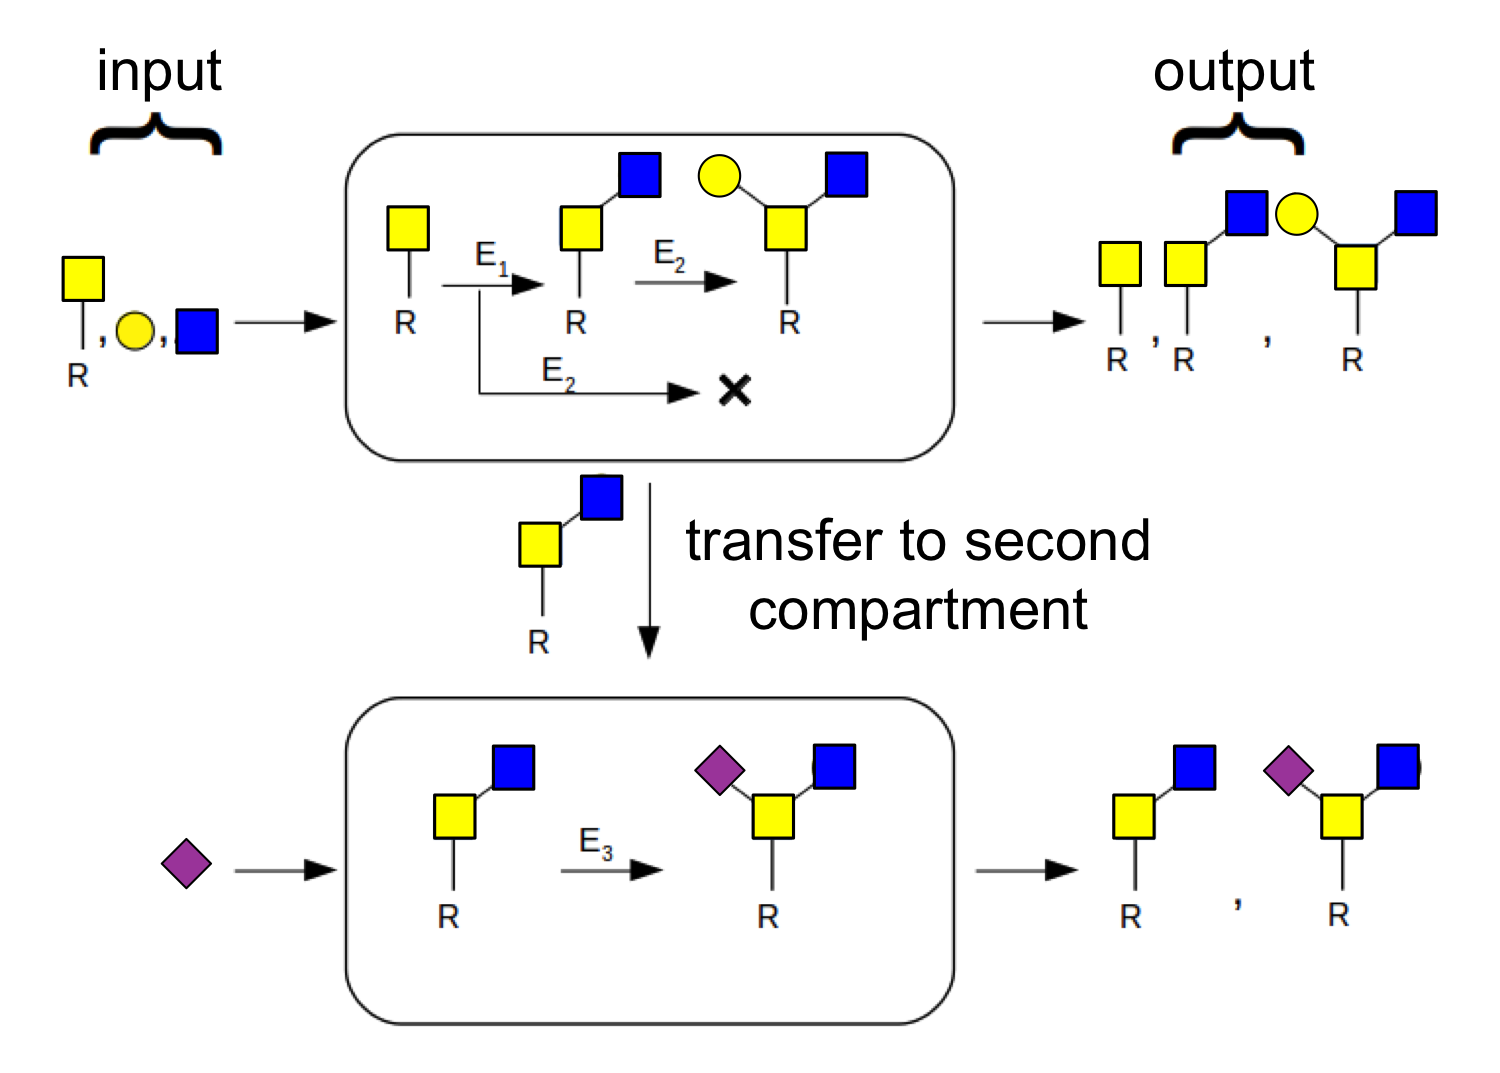
\includegraphics[width=0.9\linewidth]{gfig1.png}    
  \end{minipage}
  \begin{minipage}{0.44\linewidth}
    \caption{Biological details of glycan production. There are many types of sugar monomer building blocks; %(each represented by standard colored shapes);
      for example, GalNAc (yellow square), GlcNAc (blue square), Galactose (yellow circle), Sialic Acid (purple diamond), Fucose (red triangle) and so on \cite{Varki2017}.}
    \label{fig:glycan-rule}
  \end{minipage}
% \vspace{-9mm}
\end{figure}

In Figure~\ref{fig:glycan-rule}, we present details of glycan production. A glycan is a tree-like sugar tree (nodes linked by edges) attached to a substrate protein at the root (labeled `R'). Distinct edge orientations correspond to covalent bonds of distinct carbons on the sugar monomer. Curved boxes represent reaction compartments within cells, which are the site of glycan production. Each step of glycan growth (black arrows) represents the addition of a single new monomer to a specific attachment point on the tree. Each such step is catalyzed by an enzyme, labeled $E_i$. At any stage of growth, the tree can exit the reaction compartment as an output. Alternatively, it can be passed to a subsequent reaction compartment for further growth driven by different enzymes. Note that the enzymatic rule is sensitive to the two monomers being linked by a bond, as well as any branches. For example, enzyme $E_2$ will add a Galactose to a GalNAc only if the GlcNAc branch is present; otherwise, the reaction will not proceed (`X'). The structures, reactions, and enzymes shown here are illustrative, and they do not correspond to any measured data set; see the following section for a real example. In biological experiments, the combined outputs of every compartment are measured; the underlying reactions must be inferred.
%The inference problem is the subject of this paper.

%--------------------- DO NOT ERASE BELOW THIS LINE --------------------------

%%% Local Variables:
%%% mode: latex
%%% TeX-master: "main"
%%% End:
